\documentclass{report}

\input{preamble}
\input{macros}
\input{letterfonts}
\usepackage{graphicx}

\title{\Huge{MAM2000W 2LA}\\Systems of Equations}
\author{\huge{Alex Cristaudo}}
\date{}

\begin{document}

\maketitle
\newpage% or \cleardoublepage
% \pdfbookmark[<level>]{<title>}{<dest>}
\pdfbookmark[section]{\contentsname}{toc}
\tableofcontents
\pagebreak

\chapter{Systems of Equations, Matrices and Vectors}
\section{Examples}


\ex{}{
 When using a search engine on the Internet, it is possible that the
 number of "hits" (web sites containing the keywords you've entered) may be very
 large. You will then have to spend a long time going through the list to decide
 which sites are useful. It would be very helpful if the search engine could rank the
 sites it has found in order of importance
The problem therefore is to find a way of assigning a rank to a site. One way
 of doing this is to determine the number of other important sites that have links
 to this site. To do this we add up the ranks of all the sites that have links to the
 site, and this sum becomes the rank of the site. If you think this through, you will
 probably soon see a snag: to determine the rank of a site, you have to know the
 ranks of all the sites linked to it.
 The problem therefore is to find a way of assigning a rank to a site. One way
 of doing this is to determine the number of other important sites that have links
 to this site. To do this we add up the ranks of all the sites that have links to the
 site, and this sum becomes the rank of the site. If you think this through, you will
 probably soon see a snag: to determine the rank of a site, you have to know the
 ranks of all the sites linked to it.
 \\ 
 \begin{center}
     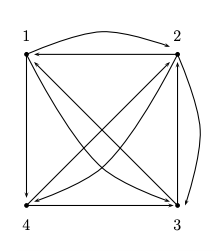
\includegraphics{img1}
 \end{center}
 An arrow from  $i$  to  $j$  indicates that site $i$  contains a link to site $j$ . Our problem is to assign a positive number $r_i$
  
 \begin{center}
$
     \begin{pmatrix} r_1 \\ r_2 \\ r_3 \\ r_4 \end{pmatrix} = k \begin{pmatrix} 0 & 1 & 1 & 0 \\ 1 & 0 & 1 & 1 \\ 1 & 1 & 0 & 1 \\ 1 & 1 & 0

 \end{pmatrix}
$
 \end{center}
 We find  $k = 0.3982$; its value is not important to us, but rather the fact
 that we get a solution for the variables $r_i$
 \\ If we write  $A$  for the matrix and $\mathbf{r}$ for the vector in this equation, it becomes $A \mathbf{r} = k^{-1}\mathbf{r}$
 \\ The number  $k^{-1}$   is an eigenvalue and vector $\mathbf{r}$ an eigenvector. So using this value for $k$ we can get $r$
}

\section{Determinants}

A determinant is a number that we associate with any
square matrix. The property of determinants that we will be primarily interested in
is the way in which it “measures” whether the matrix is invertible or not. We’ll see
that the determinant of a square matrix is 0 if and only if it is not invertible. From
a numerical point of view the determinant is also useful. It turns out that if the
absolute value of the determinant is small, then the matrix can be difficult to work
with when it comes to solving systems of equations with the matrix as coefficient
matrix

\nt{
We can think of a 2 × 2 matrix as a function from the plane $\mathbb{R}^2$
into itself: every
point in $\mathbb{R}^2$ has a position vector, and if we multiply this vector by the matrix,
we get another 2-vector, which we can think of as the position vector of a point in
the plane. It can be shown that determinants can be used to measure the factor
by which a 2 × 2 matrix (considered as such a function) will scale the area of a
region in the plane. The same is true for 3 × 3 matrices and volumes. This lies
behind the use of a special determinant, called a Jacobian
}

The notation used is $\det (A)$ or  $|A|$

\dfn{}{
    We will define determinants recursively. If $A = (a)$, then $\det(A) = a$ ($A$ is a  $1 \times 1$ matrix) \\ 
    \begin{itemize}
        \item If we delete the $i$th row and  $j$th column of $A$, the determinant of the resulting matrix is called the  $(i,j)$th minor of  $A$ (denoted by  $M_{ij})$. So if  $A$ is an  $n \times n$ matrix, $M_{ij}$ will be the determinant of an  $(n-1) \times (n-1)$ matrix
        \item The number $(-1)^{i+j}M_{ij}$ is called the  $(i,j)$th cofactor of  $A$ (denoted by  $C_{ij}$)

    \end{itemize}

Then the determinant of $A$ is defined by:
\begin{center}
\[
    \begin{aligned}
        \det (A)  & = a_{11}C_{11} + a_{12}C_{12} + \ldots + a_{1n}C_{1n}
                  &  = \sum_{j=1}^{n} a_{1j} C_{1j}
    \end{aligned}
\]
\end{center}
}


\nt{This is referred to as the expansion of $\det (A)$ along the first row}

\ex{}{
    If $A = \begin{pmatrix} a_{11}  & a_{12} \\ a_{21} & a_{22} \end{pmatrix} $, then $|A| = \det (A) = a_{11}C_{11}+a_{12}C_{12} = a_{11}a_{22} - a_{12}a_{21}$
}
\ex{}{
If $A = \begin{pmatrix} a_{11} & a_{12} & a_{13} \\ a_{21} & a_{22} & a_{23}\\a_{31} & a_{32} & a_{33} \end{pmatrix} $ 
\\ We get that $M_{11} =  \begin{vmatrix}
    a_{22} & a_{23} \\ a_{32} & a_{33}
\end{vmatrix}, M_{12}=\begin{vmatrix}
    a_{21} & a_{23}\\a_{31} & a_{33}
\end{vmatrix}, M_{13}=\begin{vmatrix}
    a_{21} & a_{22}\\a_{31} & a_{32}
\end{vmatrix}$  \\ and $C_{11}=M_{11}, C_{12}=-M_{12}, C_{13} = M_{13}$ 
\\ ~\\
Using this to work out: $\begin{vmatrix}
    2 & 3 & 1 \\ 5 & 3 & 0 \\ 7 & 6 & 4
\end{vmatrix} = 2\begin{vmatrix}
    3 & 0 \\ 6 & 4
\end{vmatrix} - 3 \begin{vmatrix}
    5  & 0 \\ 7  & 4
\end{vmatrix} + 1 \begin{vmatrix}
    5  & 3 \\ 7 & 6
\end{vmatrix} = -27$
}

Now we state 2 properties of determinants (but without the proofs):
\mprop{}{
Let $A$ be an  $n \times n$ matrix. Then 
\begin{center}
    $ \det (A) = a_{11}C_{11}+a_{21}C_{21}+ \ldots+a_{n1}C_{n1} = \sum_{i=1}^{n} a_{i1} C_{i1}$
\end{center}
}
So we can expand along the first column as well

\cor{}{
If $A$ is a square matrix, then  $\det (A^T) = \det (A)$
}
\nt{A corollary to a proposition or a theorem is a result that can easily be deduced from the proposition or theorem}

\mprop{}{
Let $A$ be a square matrix and  $B$ be the matrix obtained by interchanging any 2 rows of  $A$. Then  
\begin{center}
    $\det (B) = -\det(A)$
\end{center}
}

\cor{}{

Let $A$ be a square matrix and  $B$ be the matrix obtained by interchanging any 2 columns of  $A$. Then
\begin{center}
    $\det (B) = -\det(A)$
\end{center}
}

\begin{myproof}
    (of the above corollary, the proposition is not proved) We use the first corollary and that interchanging 2 columns in $A$ is the same as interchanging 2 rows in  $A^T$
\end{myproof}

\thm{}{
Let $A$ be an  $n \times n $ matrix. Then
\begin{itemize}
    \item $\det (A) = \sum \limits _{j=1}^{n} a_{ij} C_{ij}$ for any $1\le i\le n$
            \\ This is called expanding $\det (A) $ along the $i$th row
        \item $\det (A) =  \sum \limits _{i=1}^{n} a_{ij} C_{ij}$
            \\ This is called expanding $\det (A)$ along the  $j$th column 
\end{itemize}
}

\begin{myproof}
    ~\\
    \begin{itemize}
        \item Let $1 < i \le n$. We can make row  $i$ the first row by interchanging adjacent rows  $i-1$ times (swapping $i$ with row  $i-1$ repeatedly). Let  $B$ be the matrix obtained in this way. We then get that $\det (B) = (-1)^{i-1} \det (A)$. Denote $A_{ij}$ for the  $(n-1) \times (n-1)$ matrix obtained by deleting the $i$th row of $A$ and $j$th column of $A$ and $B_{ij}$ for $B$. It follows that  $A_{ij} = B_{1j} $ (why we do the adjacent swaps, order of the rest of the matrix is preserved) and also  $a_{ij} = b_{1j}$. Hence
            \begin{center}
                \[
            \begin{aligned}
                \det (A) = (-1)^{i-1}\det (B) & = (-1)^{i-1} \sum_{j=1}^{n} b_{1j} \det (B_{1j}) \\
                                            & = (-1)^{i-1} \sum_{j=1}^{n} (-1)^{1+j}a_{ij} \det (A_{ij}) \\
                                            & = \sum_{j=1}^{n} (-1)^{i+j}a_{ij} \det (A_{ij}) \\
                                            &  = \sum_{j=1}^{n} a_{ij}C_{ij}
            \end{aligned}
                \]
            \end{center}
        \item We could use the fact that expanding along column $j$ is equivalent to expanding along row  $j$ in  $A^T$.  But we proved we can and $\det (A) = \det (A^T)$ 
    \end{itemize}
\end{myproof}

\newpage 
\thm{}{
Let $A$ be an  $n \times n$ matrix.
\begin{enumerate}
    \item If $A$ is a triangular matrix (upper or lower), then  $\det (A) = a_{11}a_{22}\ldots a_{nn}$
    \item If a row or column of $A$ has zeroes only, then  $\det (A) = 0$
    \item If  $A$ has 2 identical rows (or columns), then  $\det (A) = 0$
    \item If a row or column of  $A$ is multiplied by a constant  $k$, then the new determinant for is  $k \det (A)$. That is, for an $n \times n$ matrix, $\det (kA) = k^n \det (A)$ 
    \item If the matrix $B$ is obtained from  $A$ by adding one row of  $A$ to \underline{another} (not the same) row of  $A$, then  $\det (B) = \det (A)$

\end{enumerate}
}

\begin{myproof}
    ~\\
    \begin{enumerate}
        \item If $A$ is lower triangular (top triangle is 0), we can expand along the first row, in which only  $a_{11}$ could be non-zero. Then the minor term can be expanded along its first row similarly. Repeating the process gives the result. Note we can do an inductive proof such as: \\
            We induct on $n$. Base case:  $n=1$ and  $A = (a_{11})$, then $\det (A) = a_{11}$ as required. Now assume, for some $n \times n$ matrix that $\det (A) = a_{11}a_{22}\ldots a_{nn}$. Now consider the following $(n+1) \times (n+1)$ matrix: \\
            Let   $(n+1) \times (n+1)$  matrix

            $ A  =
            \begin{pmatrix}
                a_{11}  & 0  & \cdots  & 0  & 0 \\
                a_{21}  & a_{22}  & \cdots  & 0  &  0 \\
                \vdots & \vdots & \ddots & \vdots  & \vdots \\
            a_{n1}  & a_{n2}  & \cdots & a_{nn}  & 0 \\
            a_{(n+1)1}  & a_{(n+1)2}  & \cdots  & a_{(n+1)n}  & a_{(n+1)(n+1)} 
            \end{pmatrix} $ \\ Expanding along the first row gives $\det (A) = a_{11} \begin{vmatrix}
            a_{22}  & 0 & \ldots & 0 \\ \vdots  &  \ddots  & \vdots  & \vdots \\ a_{n2}  & \ldots  &  a_{nn}  & 0 \\   a_{(n+1)2}  & \cdots  & a_{(n+1)n}  & a_{(n+1)(n+1)}
        \end{vmatrix} = a_{11}(a_{22}a_{33}\ldots a_{nn}) $ by the inductive hypothesis, since $C_{11}$ is an $n \times n$ matrix which completes the proof 
        An upper triangular matrix's transpose is lower which completes that part of the proof

    \item We expand along the row or column of zeroes
    \item Let $B$ be the matrix obtained from  $A$ by interchanging the two identical rows (or columns). We get that  $\det (B) = -\det (A)$ but  $A=B$, so we must have that  $\det (B)=\det (A) = 0$.
    \item Expanding along the row multiplied by  $k$ gives the result. The second part is proven by multiplying each row by  $k$ to get  $kA$, thus multiplying the determinant by  $k^n$ 
    \item Suppose we add $R_i \to R_i + kR_j$ to obtain matrix  $B$ from  $A$. Thus in row  $i$, every element is in the form  $a_{im} + ka_{jm}$. Expanding  $\det (B)$ along this row gives:
         \begin{center}
            \[
            \begin{aligned}
                \det (B) & = \sum_{m=1}^{n} b_{im}C_{im} \\ 
                         & = \sum_{m=1}^{n} (a_{im} + ka_{jm})C_{im} \text{ and note $C_{im}$ is the same  $C_{im}$ as used in  $\det (A)$} \\
                         & = \sum_{m=1}^{n} a_{im}C_{im} + k\sum_{m=1}^{n} a_{jm}C_{im}
                        \\ \text{Now if } C \text{ is obtained by replacing row }   &  i \text{ with row }  j \text{, this becomes: }\\ 
                         & = \sum_{m=1}^{n} a_{im}C_{im} + k\sum_{m=1}^{n} c_{im}C_{im} \\ 
                         &  = \det (A) + k\det (C)  \text{ but } C \text{ has two identical rows, so} \\
                          & = \det (A) + 0 = \det (A)
            \end{aligned}
            \]
        \end{center}
    \end{enumerate}
\end{myproof}

\thm{}{
    Let $E$ be an elementary matrix. 
     \begin{enumerate}
        \item If $E$ is associated with adding a multiple of one row to another row, then  $\det (E) = 1$
        \item If  $E$ is associated with a row interchange, then  $\det (E) = -1$
        \item If  $E$ is an elementary matrix associated with multiplication of  row  $i$ by a non-zero \underline{constant} $k$, then  $\det (E) = k$
        \item For any elementary matrix  $E$ and any $n \times n$ matrix $A$, we get  $\det (EA) = \det(E) \det(A)$
    \end{enumerate}
}

\begin{myproof}
    ~\\
    \begin{itemize}
        \item This follows from the fact in this case, $E$ is either upper or lower triangular with  $e_{ii} = 1$ for $1 \le i \le n$.
         \item $E$ is obtained by interchanging two rows of  $I$, so  $\det (E) = -\det (I) = -1$
         \item  $E$ differs from  $I$ by having $k$ in position $(i,i)$. So $\det (E) = k\det(I) = k$
         \item You can see that this is true for the elementary matrices that correspond to row
interchange or multiplication of a row by a non-zero constant. We know that in the
case of a row interchange, the associated elementary matrix has determinant $-1$,
and that interchanging two rows multiplies the determinant of any matrix by $-1$.
In the case that we are multiplying a row of a matrix by a non-zero constant $k$,
we already know that this multiplies the determinant of the matrix by $k$, and $k$ is
also the determinant of the associated elementary matrix. In the case that the row
operation involves adding a multiple of one row to another row, the determinant
of the resulting matrix is unchanged and $\det (E) = 1$, from
which the result follows
    \end{itemize}
\end{myproof}

\ex{}{
$\begin{vmatrix}
    1  & 2 \\ 3  & 4
\end{vmatrix} = -2$. \\ Now if perform operation $R_2 \to R_2 + 2R_1$, we get matrix  $\begin{pmatrix} 1  & 2 \\ 5 & 8 \end{pmatrix} $ which also has determinant $-2$
} 

We are now in a position to link up the idea of a determinant to invertibility of
a matrix. (We can't really claim to prove the result, since our "proof" depends on
results about determinants which we have not all proved here.)

\thm{}{
    Let $A$ be a square matrix. Then  $\det (A) \ne 0 \iff A$ is invertible
}
\begin{myproof}
    Assume $A$ is invertible, then  $A = E_kE_{k-1}\ldots E_1$ where each $E_i$ is elementary \\ Now  $\det(A) = \det(E_k) \det (E_{k-1}) \ldots \det (E_1) \ne 0$ since we know that $\det (E) = \begin{cases}
        1 & \text{ for adding a multiple of one row to another} \\ -1 &  \text{ for interchanging rows} \\ k &  \text{ for multiplying my constant }k
    \end{cases}$ which is never $0$ \\ Conversely, assume  $\det (A) \ne 0.$ Since  $A$ is row equivalent to some row echelon form  $U$, we get  $A = E_k E_{k-1} \ldots E_1 U \implies \det (U) \ne 0$ and thus none of the entries on diagonal  $U$ are zero, so  $U$ is row equivalent to  $I$ meaning  $A$ is row equivalent to  $I$ and thus invertible
    \nt{We can add the condition $\det (A) \ne 0$ to the invertibility theorem}
\end{myproof}

\dfn{Eigenvectors and Eigenvalues}{
    Let $A$ be a square matrix. A scalar  $ \lambda $ is called an eigenvalue of $A$ if there exists vector  $\mathbf{x} \ne \mathbf{0}$ such that $A \mathbf{x} = \lambda \mathbf{x}$. The non-zero vector $\mathbf{x}$ is called an eigenvector corresponding to eigenvalue $ \lambda $
}

Determinants help us find eigenvalues:

\thm{}{
    Let $A$ be a square matrix. Then  $ \lambda $ is an eigenvalue of $A \iff \det( \lambda I - A) = 0$
}

\begin{myproof}
    First note that $A \mathbf{x} = \lambda \mathbf{x} \iff \left( \lambda I - A \right) \mathbf{x} = \mathbf{0}$ . \\ There is a non-zero vector $\mathbf{x}$ such that $\left( \lambda I - A \right) \mathbf{x} = \mathbf{0} \iff \lambda I - A$ is singular, that is, $ \lambda I - A$ is not invertible $ \iff \det ( \lambda I-A) = 0$
\end{myproof}

\thm{}{
Let $A$ and  $B$ be $n \times n$ matrices, then \\ 
$\det (AB) = \det(A) \det (B)$
}
\begin{myproof}
    We consider two mutually exclusive cases:
    \begin{itemize}
        \item Assume $A$ is singular, then so is  $AB$ so  $\det (A) \det (B) = 0 \times \det(B) = 0 = \det (AB)$
        \item Assume $A$ is non-singular, then $A = E_k E_{k-1} \ldots E_1$, then $\det (AB) = \det \left( E_k E_{k-1}\ldots E_1 B \right)  = \det (E_k) \ldots \det(E_1) \det(B) = \det(A) \det(B)$
    \end{itemize}
\end{myproof}

\cor{}{
    Let $A$ be a square matrix such that  $\det (A) \ne 0$, then  $\det (A^{-1}) = \frac{1}{\det (A)}$
}
\begin{myproof}
    $\det (A^{-1}) \det (A) = \det (A^{-1}A) = \det (I) = 1$
\end{myproof}

\ex{}{Get example for computing determinants quicker}

\nt{
Warning: Do not fall into the trap of thinking that row reducing a matrix to its
row echelon form and then finding the determinant of the row reduced form will
give you the determinant of the original matrix. You can see, for instance, from
the above example that each row interchange used will introduce a factor of -1.
Similarly, multiplying a row by a constant would also introduce a new factor.
}

\thm{Cramer's Rule}{
Let $A$ be an invertible  $n \times n$ matrix and $\mathbf{b} \in \mathbb{R}^n$. Then the system $A \mathbf{x} = \mathbf{b}$ has a unique solution given by \\
\begin{center}
    $x_k = \frac{\det (A_k[\mathbf{b}])}{\det (A)}$ for $k=1,2,\ldots,n$
\end{center}
}
\begin{myproof}
    Using the fact that $A \mathbf{x} = \mathbf{b} $ it can be checked that $AI_k [\mathbf{x}] = A_k [\mathbf{b}]$ \\ This implies that $\det (A) \det (I_k [\mathbf{x}]) = \det (AI_k [\mathbf{x}]) = \det (A_k [\mathbf{b}])$. Since $\det (I_k [\mathbf{x}])=x_k$, the result follows
\end{myproof}
\end{document}
